%%%%%%%%%%%%%%%%%%%%%%%%%%%%%%%%%%%%%%%%%%%%%%%%%%%%%%%%%%%%%%%%%%%%%%%%%%%%%%%% 

\documentclass[%
	25pt, 
	a0paper, 
	portrait, 
	margin=0mm, 
	innermargin=25mm,
	blockverticalspace=10mm, 
	colspace=25mm,
	subcolspace=0mm
]{tikzposter}

\usepackage{amsfonts,amssymb,amsmath}
\usepackage[english]{babel}
\usepackage[T1]{fontenc}
\usepackage[utf8]{inputenc}
\usepackage{lmodern}
\usepackage[skins]{tcolorbox}
\usepackage[absolute,overlay]{textpos}
\usepackage[percent]{overpic}
\usepackage{marvosym}
\usepackage{epstopdf}
\usepackage{enumitem}
\usepackage{color}
\usepackage{tikz}
\usepackage{lipsum}

\renewcommand{\familydefault}{\sfdefault}
\bibliographystyle{plain}

\tikzposterlatexaffectionproofoff

%%%%%%%%%%%%%%%%%%%%%%%%%%%%%%%%%%%%%%%%%%%%%%%%%%%%%%%%%%%%%%%%%%%%%%%%%%%%%%%% 

% Define RWTH Aachen University colors
\definecolor{rwthdarkblue}{RGB}{0,84,159}
\definecolor{rwthlightblue}{RGB}{142,186,229}
\definecolor{rwthdarkgray}{RGB}{100,101,103}
\definecolor{rwthlightgray}{RGB}{236,237,237}

\definecolor{rwthmagenta}{RGB}{227,0,102}
\definecolor{rwthyellow}{RGB}{255,237,0}
\definecolor{rwthpetrol}{RGB}{0,97,101}
\definecolor{rwthturquoise}{RGB}{0,152,161}
\definecolor{rwthgreen}{RGB}{87,171,39}
\definecolor{rwthmaygreen}{RGB}{189,205,0}
\definecolor{rwthorange}{RGB}{246,168,0}
\definecolor{rwthred}{RGB}{204,7,30}
\definecolor{rwthbordeauxred}{RGB}{161,16,53}
\definecolor{rwthviolet}{RGB}{97,33,88}
\definecolor{rwthpurple}{RGB}{122,111,172}


% Set colors within tikzposter class
\colorlet{titlebgcolor}{white}
\colorlet{framecolor}{white}
\colorlet{blocktitlefgcolor}{white}
\colorlet{blocktitlebgcolor}{rwthdarkblue}
%\colorlet{blocktitlebgcolor}{gray}
\colorlet{innerblockbodyfgcolor}{white}
\colorlet{backgroundcolor}{white}

% TITLE

\newlength{\boxw}
\newlength{\boxh}
\newlength{\tmpa}
\newlength{\depth}
\newlength{\shadowsize}

\setlength{\depth}{6pt}
\setlength{\shadowsize}{5pt}

\definetitlestyle{grktitle}{
	width=350mm,
	roundedcorners=0pt, 
	linewidth=0pt, 
	innersep=5pt,
	titletotopverticalspace=25mm, 
	titletoblockverticalspace=25mm
}{
	\setlength{\boxw}{\titleposright - \titleposleft}
	\setlength{\boxh}{\titlepostop - \titleposbottom}
	\foreach \x in {0,.1,...,1}
	{
		\setlength{\tmpa}{\shadowsize * \real{\x}}
 		\fill[shift={(\titleposleft+\depth,\titlepostop-\depth)},
 				black, opacity=.05, rounded corners=\tmpa]
			(-\tmpa,\tmpa) rectangle +(\boxw+2*\tmpa,-\boxh-2*\tmpa);
	}
	\filldraw[fill=white!50, draw=white!50, rounded corners=\titleroundedcorners]
		(\titleposleft, \titlepostop) rectangle (\titleposright, \titleposbottom);
}

% Compactify the bibliography
\let\oldbibliography\thebibliography
\renewcommand{\thebibliography}[1]{%
\scriptsize
   \oldbibliography{#1}%
   \setlength{\itemsep}{2pt}%
   \setlength{\parskip}{0pt}%
}

\settitle{ \centering \fontsize{100}{70} \vbox{ \@titlegraphic \\
[\TP@titlegraphictotitledistance] \centering
\color{titlefgcolor} {\bfseries   \@title \par}
\vspace*{2em}
{\Large \@author \par} \vspace*{1em} {\large \@institute}
}}

% Change block border style
\newcommand{\myblock}[2]{\block[titleinnersep=4mm, bodyinnersep=10mm, titlewidthscale=1.05, bodywidthscale=1.05, roundedcorners=8, linewidth=3pt]{#1}{#2}}

% Define a no border block style
\newcommand{\noborderblock}[2]{
	\colorlet{blocktitlebgcolortmp}{blocktitlebgcolor}
	\colorlet{blocktitlebgcolor}{white}
	\myblock{#1}{#2}
	\colorlet{blocktitlebgcolor}{blocktitlebgcolortmp}
}

%%%%%%%%%%%%%%%%%%%%%%%%%%%%%%%%%%%%%%%%%%%%%%%%%%%%%%%%%%%%%%%%%%%%%%%%%%%%%%%% 

% Set title, author and affiliation
\title{Your title}
\author{\bfseries \textcolor{rwthdarkgray}{First author *) and second author **)}}
\institute{\bfseries \textcolor{rwthdarkgray}{*) Chair of Methods for Model-based Development in Computational Engineering, RWTH Aachen University}\\[0.5cm]
\textcolor{rwthdarkgray}{**) Chair of Methods for Model-based Development in Computational Engineering, RWTH Aachen University}}


\begin{document}

%Logo
\node [below=4cm, left=1cm] at (topright) {
\includegraphics[width=0.5\linewidth]{logo/Logo_rwth_mbd_en_rgb.png}};

\maketitle[width=31.9in,roundedcorners=0,titletotopverticalspace=8cm,titletoblockverticalspace=0cm]

%%%%%%%%%%%%%%%%%%%%%%%%%%%%%%%%%%%%%%%%%%%%%%%%%%%%%%%%%%%%%%%%%%%%%%%%%%%%%%%% 

\begin{columns}
 
 % FIRST column
\column{0.33}
\myblock{Block 1}{
  \large{\lipsum[1]}\\

  \begin{center}
    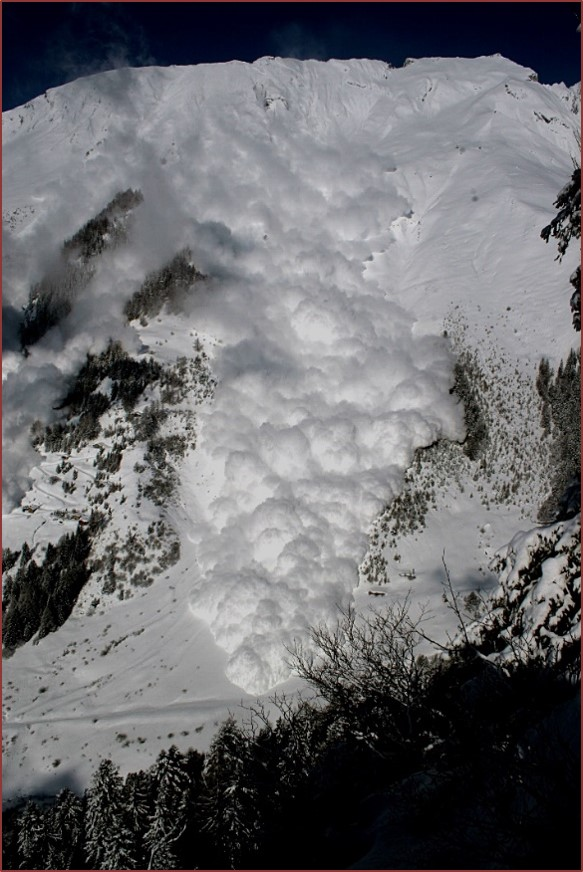
\includegraphics[height=0.6\linewidth]{figures/lawine.jpg} \qquad
    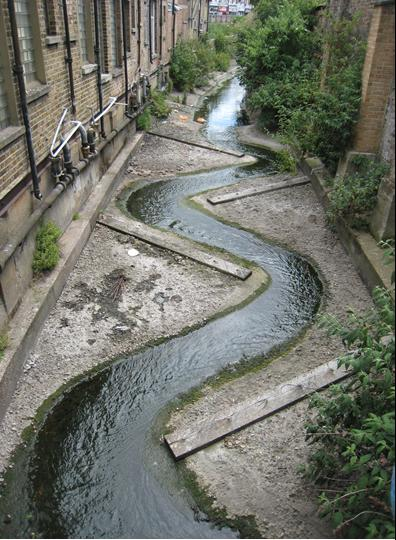
\includegraphics[height=0.6\linewidth]{figures/LowFlow.jpg}\\[0.5cm]
  \end{center}
}

\myblock{Block 2}{
  \large{\lipsum[1]}

  \large{Equation 1: }
  \normalsize{
    \begin{equation*}
      \begin{aligned}
        1+1=2
      \end{aligned}
    \end{equation*}}
}


\myblock{Block 3}{
  \begin{itemize}
    \item Item 1
    \item Item 2
    \item Item 3
    \item Item 4
    \item Item 5
  \end{itemize}
}




	
% MIDDLE column
\column{0.33}
\myblock{Block 4}{
  \large{\lipsum[1]}\\
}

\myblock{Block 5}{
  \large{\lipsum[1]}\\
}

\myblock{Block 6}{
  \large{\lipsum[1]}\\
}






% RIGHT column
\column{0.33}
\myblock{Block 7}{
  \large{\lipsum[75]}\\
}

\myblock{Block 8}{
  \large{\lipsum[5]}\\
}

\myblock{Block 9}{
  \large{\lipsum[6]}\\
}

\myblock{Block 10}{
  \large{\lipsum[8]}\\
}

\myblock{Block 11}{
  \large{\lipsum[75]}\\
}






	
\end{columns}

% Authors, acknowledgments and references 
\column{0.5}

\begin{columns}
	\column{0.088}
	\column{0.25}
	\noborderblock{}{
		\vspace{-1em}
        \begin{minipage}[c]{0.2\linewidth}
          
\includegraphics[width=\linewidth]{figures/author1.jpg}
        \end{minipage}
        \hspace{1mm}
        \begin{minipage}{0.8\linewidth}
            Author 1\\
            \Letter\hspace{3mm}author1@mbd.rwth-aachen.de	
        \end{minipage}
        
        \vspace{2mm}
        
        \begin{minipage}{0.2\linewidth}
          
\includegraphics[width=\linewidth]{figures/author2.jpg}
        \end{minipage}
        \hspace{1mm}
        \begin{minipage}{0.8\linewidth}
            Author 2\\
            \Letter\hspace{3mm}author2@mbd.rwth-aachen.de
        \end{minipage}
        
        % \vspace{2mm}
		% \small {\footnotesize \textbf{Acknowledgments}
		% The project is supported by nobody}
		% \hfill
	}
	
	\column{0.645}

\myblock{References}{
	%\vspace*{-1em}
%	\renewcommand{\refname}{~}
	\begin{enumerate}[label={[\arabic*]}]
	\item Ref 1
	\item	Ref 2	
	\end{enumerate}
}
\end{columns}


\end{document}

%%%%%%%%%%%%%%%%%%%%%%%%%%%%%%%%%%%%%%%%%%%%%%%%%%%%%%%%%%%%%%%%%%%%%%%%%%%%%%%% 
